%% AI-Assisted 3D Assembly Design -- conference paper
%% Built on the Springer Nature sn-jnl template (sn-mathphys, Numbered references).
%% Compile in the GL-provided Overleaf project: set the main file to this one,
%% and keep sn-bibliography.bib alongside it (already updated with this paper's
%% references -- do not reuse the template's original sample .bib).

\documentclass[sn-mathphys,Numbered]{sn-jnl}

\usepackage{graphicx}%
\usepackage{multirow}%
\usepackage{amsmath,amssymb,amsfonts}%
\usepackage{amsthm}%
\usepackage{mathrsfs}%
\usepackage[title]{appendix}%
\usepackage{xcolor}%
\usepackage{textcomp}%
\usepackage{manyfoot}%
\usepackage{booktabs}%
\usepackage{algorithm}%
\usepackage{algorithmicx}%
\usepackage{algpseudocode}%
\usepackage{listings}%

\raggedbottom

\begin{document}

\title[GNNs for CAD Assembly Completion]{Graph Neural Networks for Missing-Component Detection, Recommendation, and Shape Generation in CAD Assemblies}

\author*[1]{\fnm{Parthasarathy} \sur{Perumal}}\email{parthasarathy.perumal@gmail.com}

\affil*[1]{\orgdiv{Student -- M.Tech Data Science and AI}, \orgname{PES University}, \orgaddress{\street{Hosur Rd, Konappana Agrahara}, \city{Bangalore}, \postcode{560100}, \state{Karnataka}, \country{India}}}

\noindent\textit{Corresponding author(s). E-mail(s): \href{mailto:parthasarathy.perumal@gmail.com}{parthasarathy.perumal@gmail.com};}

\abstract{Modern CAD tools offer no contextual intelligence during assembly creation: engineers rely entirely on domain experience to decide which components an assembly still needs and where they belong. We present an end-to-end graph neural network (GNN) system that treats a mechanical assembly as an attributed graph -- solid bodies as nodes, real contact surfaces as edges -- and addresses assembly completion in two phases. Phase~I detects missing components via inductive link prediction over a shared relational-attention encoder (RGATConv). Phase~II recommends the most likely next component type through a learned ranking head, then generates an actual placeable 3D shape for it through a hybrid retrieval-plus-conditional-VAE generator, rather than only a text label. Both phases build on a single frozen Phase~I encoder, so the marginal cost of each new task head is small. On a curated corpus of 749 CAD assemblies spanning seven machine-part categories (648 usable graphs, 25{,}155 labelled bodies after parsing), the system reaches a mean link-prediction AUC-ROC of 0.9206 ($\pm$0.0121) and mean average precision of 0.9020 across true five-fold cross-validation, a next-component ranking Hit@1 of 0.4093 against a majority-class baseline of 0.3442, and a shape-generation test IoU of 0.6459 with a Chamfer distance of 0.0377. We further contribute a novel Octree-based open-surface detector for locating candidate mating joints without a CAD kernel, an assembly-template frequency prior that works even from a single uploaded body, and an interactive natural-language explanation layer built on GNNExplainer attributions. We report an engineering finding from exploratory analysis of the current corpus -- a silently dead shape-descriptor feature affecting 99.95\% of bodies -- as a reminder that dataset-level auditing remains essential even after a model trains successfully.}

\keywords{Graph Neural Networks, CAD Assembly, Link Prediction, Component Recommendation, Shape Generation, Variational Autoencoder, Relational Attention}

\maketitle

\section{Introduction}\label{sec:intro}

Assembling a mechanical design in a modern CAD package -- SolidWorks, CATIA, Fusion~360 -- is still a manual, expert-driven process. The software tracks geometry and mating constraints faithfully, but it offers no judgement about the assembly itself: it cannot tell a designer that a bolted joint is missing its nut, that a valve housing typically pairs with a particular gland-plate variant, or what shape a plausible replacement part should take. That judgement lives entirely in the designer's experience. For junior engineers, or for anyone auditing a partially-defined assembly inherited from someone else, this is a real productivity and quality gap: incomplete assemblies have no built-in mechanism to flag what is missing, and no standardised way to suggest what should be added.

This gap is a natural fit for graph-based deep learning. A rigid mechanical assembly is, structurally, a graph: solid bodies are nodes, and physical contact between two bodies -- a bolt seated in a hole, a shaft running through a bushing -- is an edge. Graph neural networks (GNNs) are designed to learn representations over exactly this kind of relational structure, and have driven substantial recent progress in adjacent CAD-generation tasks such as boundary-representation (B-Rep) synthesis \cite{brepgen2024,solidgen2024} and construction-sequence generation from language \cite{cadgpt2025}. Those systems generate whole shapes or whole sequences; comparatively little work targets the narrower, more directly actionable problem this paper addresses: given a \emph{partial} real assembly, what is missing, what should be added next, and what should it look like.

Framing assembly completion this way raises three practical requirements that shape every design choice in this paper. First, the system must work from geometry a designer can actually produce -- a STEP export -- rather than from a synthetic or hand-labelled graph, which pushes real engineering weight onto the feature-extraction pipeline (Section~\ref{sec:graphconstruction}) rather than only the model. Second, detection, recommendation, and generation are three different kinds of prediction (an edge score, a categorical ranking, a continuous 3D shape), and training three unrelated models from scratch would triple the data and compute burden for a corpus that, by the standards of large-scale shape datasets \cite{koch2019abc,mo2019partnet}, is modest; sharing one encoder across all three tasks is a deliberate response to that constraint, not merely an implementation convenience. Third, an incorrect but confident suggestion is arguably worse than no suggestion at all in an engineering context, which motivates both the retrieval-first bias in Section~\ref{sec:shapegen} (a real, imperfect part is preferred over a plausible-looking hallucination) and the explanation layer in Section~\ref{sec:novel} (a suggestion the designer cannot audit is one they should not trust).

We treat assembly completion as two connected phases built on one shared encoder. \textbf{Phase~I} is a missing-component \emph{detection} problem, framed as inductive link prediction over the assembly graph: score candidate body pairs for whether a real mating connection should exist between them, and a body with an unusually low-scoring, unmatched candidate connection is flagged as a probable missing part. \textbf{Phase~II} is a \emph{completion} problem in two steps -- rank which of eight canonical component types most plausibly fills a detected gap, then generate an actual 3D shape for it, first by retrieving a close match from a bank of parts seen during training, falling back to a small conditional variational autoencoder (VAE) only when no good match exists. Both phases reuse the same relational-attention encoder trained once for Phase~I and then frozen, so each new task head is a comparatively cheap addition rather than a full new model.

This paper makes the following contributions:
\begin{itemize}
\item An end-to-end GNN pipeline -- detect, rank, generate -- that operates directly on STEP-derived assembly graphs with a 34-dimensional geometric node feature vector and a 6-dimensional contact-edge feature vector, requiring no proprietary CAD-kernel API at inference time.
\item A hybrid shape generator that prefers real retrieved geometry over a generative fallback, and a corresponding evaluation showing this materially outperforms VAE-only generation on both intersection-over-union and Chamfer distance.
\item Two supporting components with no analogue in the CAD-generation literature we surveyed: an Octree-based open-surface detector that locates candidate joint locations from raw mesh geometry alone, and a per-category component-type frequency prior (\textit{AssemblyTemplateDB}) that produces a useful completion signal even from a single uploaded body with no graph context at all.
\item A GNNExplainer-based, natural-language explanation layer that turns raw attribution scores into engineering-readable justifications for each prediction, evaluated live against real uploaded STEP files.
\item A transparent account of two engineering findings surfaced during development -- a previously silent, all-zero feature dimension found only through exploratory data analysis of the final training corpus, and a majority-class bias in the ranking head -- reported here in the interest of reproducibility rather than omitted for polish.
\end{itemize}

The rest of this paper is organised as follows. Section~\ref{sec:related} surveys related work in CAD generation and graph representation learning. Section~\ref{sec:arch} describes the shared graph-construction pipeline and encoder. Sections~\ref{sec:phase1} and \ref{sec:phase2} detail Phase~I detection and Phase~II recommendation/generation respectively. Section~\ref{sec:novel} covers the two supporting contributions. Section~\ref{sec:setup} describes the experimental corpus and protocol, Section~\ref{sec:results} reports results and the two engineering findings, and Section~\ref{sec:conclusion} concludes with limitations and future work.

\section{Related Work}\label{sec:related}

\textbf{Generative CAD models.} Recent work generates CAD geometry directly: BrepGen \cite{brepgen2024} uses a structured latent diffusion model to synthesise valid B-Rep solids; SolidGen \cite{solidgen2024} is an autoregressive model over B-Rep topology and geometry; CAD-GPT \cite{cadgpt2025} synthesises CAD construction sequences from natural-language spatial reasoning. All three generate individual parts or full designs from a specification or a prior distribution. None of them consume a partially-built \emph{assembly} and reason about what specific component is missing from it -- the problem this paper addresses is complementary, not competing.

\textbf{GNNs for structural and link-level reasoning.} Graph convolutional and attention architectures \cite{kipf2017gcn,velickovic2018gat,hamilton2017sage} established the modern toolkit for learning over irregular relational data, and relational-attention variants such as RGATConv \cite{busbridge2019rgat} extend attention with per-edge-type parameters -- the mechanism this work builds on directly, since a mechanical joint's type (rigid, revolute, slider, cylindrical) materially changes how two connected bodies should influence each other's representation. A recent theoretical analysis questions how much of standard link-prediction performance is attributable to simple structural heuristics rather than learned features \cite{linkheuristics2024}; our node features are dominated by affine-invariant shape descriptors rather than pure topology, which should make the encoder less susceptible to that failure mode, though we do not claim to have isolated the effect. Heterogeneous graph contrastive learning \cite{heterognn2023} is a related but self-supervised alternative to the supervised link-prediction and ranking objectives used here.

\textbf{CAD/mechanical part datasets.} Large open datasets such as ABC \cite{koch2019abc} and PartNet \cite{mo2019partnet} have been central to progress in learned shape understanding, but both are dominated by consumer and generic-object geometry rather than the industrial fastener- and joint-heavy assemblies (vices, valves, hooks, presses) this system targets; we build and curate our own corpus for that reason, described in Section~\ref{sec:setup}.

\textbf{Interpretability.} GNNExplainer \cite{ying2019gnnexplainer} produces post-hoc subgraph and feature attributions for a trained GNN's prediction. We use it as the numerical backbone for Section~\ref{sec:novel}'s explanation layer, translating its attribution scores into natural-language engineering justifications rather than presenting them as raw importance weights.

\textbf{Graph representation choices.} Shallow, structure-only embedding methods such as node2vec \cite{grover2016node2vec} learn node representations from random-walk co-occurrence alone, with no mechanism to consume continuous node or edge attributes. For an assembly graph whose nodes carry rich geometric descriptors (Section~\ref{sec:graphconstruction}) and whose edges carry a physically meaningful joint-type label, discarding that information would be a significant loss of signal; this motivates the attention-based, feature-and-structure-aware encoder in Section~\ref{sec:encoder} over a purely structural alternative.

\textbf{Ranking and generative objectives.} The Phase~II ranking head is trained with Bayesian Personalised Ranking (BPR) \cite{rendle2009bpr}, originally proposed for implicit-feedback recommendation and adopted here because next-component recommendation is structurally the same problem: rank a small set of candidates given an incomplete context, with only relative (not absolute) preference labels available per assembly. The shape-generation fallback is a conditional variational autoencoder \cite{kingma2014vae} operating on a voxel occupancy grid, following the representation used by 3D-R2N2 \cite{choy2016occupancy} for single/multi-view 3D reconstruction, conditioned here on the frozen encoder's context vector instead of an image.

\section{System Architecture}\label{sec:arch}

Figure~\ref{fig:pipeline} summarises the full pipeline: a STEP file is converted to an attributed graph, encoded once by a shared relational-attention network, and consumed by three task heads plus a live explanation layer, with two supporting geometric modules feeding candidate-location evidence back into the encoder's input.

\begin{figure}[h]
\centering
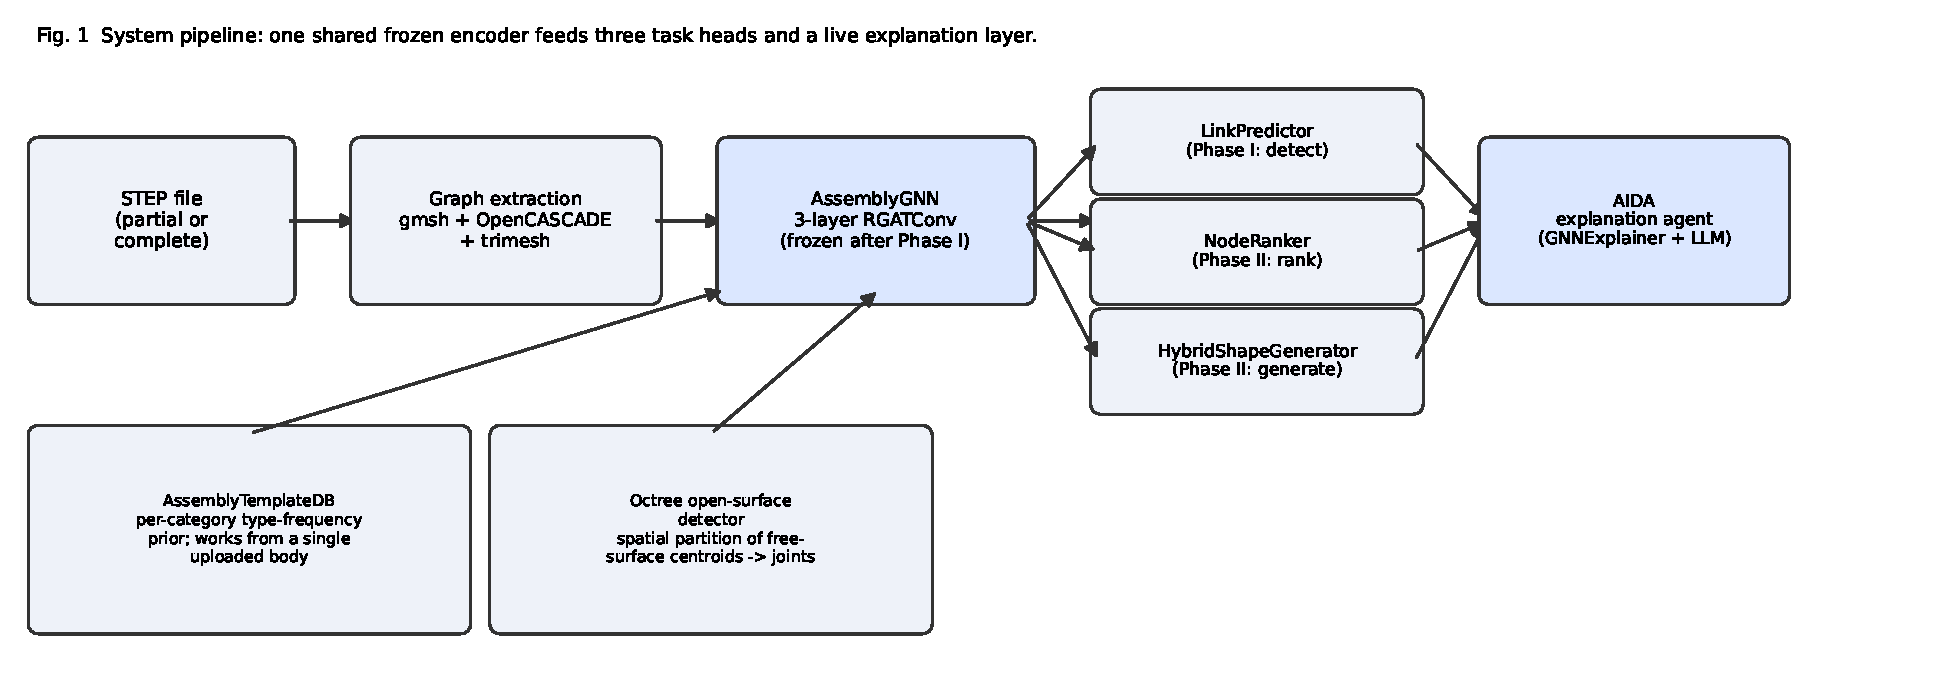
\includegraphics[width=\textwidth]{fig_pipeline.pdf}
\caption{System pipeline: one shared frozen encoder feeds three task heads and a live explanation layer.}
\label{fig:pipeline}
\end{figure}

\subsection{Graph construction}\label{sec:graphconstruction}

Each STEP assembly file is parsed with \texttt{gmsh} (OpenCASCADE kernel), fragmented into individual solid bodies, and converted into an attributed graph: one node per solid body, one edge per pair of bodies whose boundary face sets physically intersect after fragmentation (a real shared contact, not spatial proximity). Two bodies with no shared boundary get no edge, however close they sit in space.

\textbf{Node features (34-dim).} Every body carries: an 8-class component-type one-hot (long/short shaft, thick/thin plate, bolt, washer, nut, body -- assigned by multi-signal geometric voting over hole detection, bolt-head detection, and absolute-size gating, replacing an earlier single-signal SDF rule); log-scaled volume and exact surface area (via \texttt{trimesh}, not a bounding-box approximation); three scale-normalised bounding-box extents; five affine-invariant shape descriptors (elongation, flatness, two aspect ratios, sphericity); Shape Diameter Function (SDF) mean and variance from inward ray-casting; a surface-area-to-volume ratio; and twelve hole-geometry descriptors added for this corpus revision -- hole count, a binary has-holes flag, through/counterbore/indentation/filled-hole fractions and their corresponding binary flags, mean and maximum hole diameter, and a flag for whether a hole's local surroundings are curved rather than flat (fasteners essentially never mount on a curved outer surface, so this distinguishes a genuine mounting hole from an incidental one).

\textbf{Edge features (6-dim).} Two dimensions encode the mate type and a real contact-area weight (the shared-surface area ratio between the two bodies, replacing an earlier hardcoded constant), and four encode a one-hot joint-type classification (rigid, revolute, slider, cylindrical) inferred from the local contact geometry.

\subsection{Shared encoder}\label{sec:encoder}

All task heads read from one shared encoder, \textit{AssemblyGNN}: a 3-layer relational graph attention network (RGATConv) with eight attention heads at the first two layers narrowing to one at the third, hidden width 128, output embedding width 64. Both the input and output projections are node-type-conditioned -- a separate linear layer per one of the eight component-type classes, dispatched by the node's own one-hot type -- and the relational attention at every layer is conditioned on the discrete joint-type argmax of each edge, so a revolute joint and a rigid joint pass different learned attention weights even between structurally identical node pairs. Continuous edge features (contact-area weight, mate-type scalar) are injected only at the first layer. The encoder is trained once, end-to-end with the Phase~I head (Section~\ref{sec:phase1}), then frozen: every subsequent head (Section~\ref{sec:phase2}) trains only its own small parameter set on top of the fixed embeddings this encoder produces.

\subsection{Implementation details}\label{sec:implementation}

Table~\ref{tab:hyperparams} lists the training configuration for each of the three stages. All three are implemented in PyTorch with PyTorch Geometric \cite{fey2019pyg} and trained on a single Apple-Silicon GPU (Metal Performance Shaders backend). Phase~I training batches graphs by a cumulative edge-count budget rather than a fixed graph count (\textit{EdgeBudgetBatchSampler}): a handful of the corpus's larger assemblies (Section~\ref{sec:corpus}) exceed 1{,}000 edges each, and relational attention's per-edge relation-weight computation scales with a batch's total edge count, not its node count, so an unbudgeted batch combining several large graphs can exceed available GPU memory even when every individual graph fits comfortably alone.

\begin{table}[h]
\caption{Training configuration by stage.}\label{tab:hyperparams}
\begin{tabular}{@{}lll@{}}
\toprule
Parameter & Phase~I (encoder) & Phase~II (heads) \\
\midrule
Optimiser & Adam & Adam \\
Learning rate & $1\times10^{-3}$ (ReduceLROnPlateau, factor 0.5) & $1\times10^{-3}$ (NodeRanker), fixed \\
Weight decay & $5\times10^{-4}$ & $1\times10^{-5}$ (NodeRanker) \\
Batch composition & edge-budgeted, cap 300 edges/batch & full-graph context per sample \\
Early-stop patience & 20 epochs (LR patience 8) & none -- fixed 30 / 60 epochs \\
Dropout & 0.3 & -- \\
Cross-validation & true 5-fold, per-fold reseeded splits & true 5-fold protocol, fold 0 reported \\
\botrule
\end{tabular}
\end{table}

\section{Phase I: Missing-Component Detection}\label{sec:phase1}

Phase~I frames missing-component detection as inductive link prediction. Given the encoder's node embeddings $z_u, z_v \in \mathbb{R}^{64}$ for a candidate body pair $(u,v)$, a two-layer MLP head scores the pair:
\begin{equation}
\text{score}(u,v) = \text{MLP}\!\left(z_u \,\Vert\, z_v \,\Vert\, \lVert p_u - p_v \rVert_2\right)
\label{eq:linkscore}
\end{equation}
where $p_u, p_v$ are the two bodies' scale-normalised bounding-box centroids and $\Vert \cdot \Vert$ denotes concatenation. The Euclidean-distance term was a deliberate late addition: without it, every node feature is affine-invariant and message passing only ever traverses \emph{real} edges, so a candidate (non-edge) pair being scored had no signal at all for "these two bodies are nowhere near each other" -- a structurally implausible pair and a plausible-but-missing one were otherwise indistinguishable to the head. Training uses \texttt{RandomLinkSplit} per graph (10\% validation / 10\% test edges, disjoint from the message-passing edges), a 1:1 hard-negative-augmented positive:negative ratio (chosen over the field's common 1:2 skew, which measurably inflates average precision independent of real ranking skill), and standard binary cross-entropy. A missing component in a real (possibly incomplete) assembly is then operationally identified as a body whose best candidate connection scores anomalously low relative to its structurally similar peers, surfaced to the user alongside the Section~\ref{sec:novel} Octree open-surface detector's independent geometric evidence.

\section{Phase II: Next-Component Recommendation and Shape Generation}\label{sec:phase2}

Phase~II answers two questions once Phase~I has flagged that something is missing: \emph{what} component type is most likely absent, and \emph{what should it look like}. Both heads reuse the frozen Phase~I encoder and train only their own parameters.

\subsection{NodeRanker: next-component recommendation}\label{sec:noderanker}

Given the embeddings of the assembly's known nodes $\{z_i\}_{i=1}^{N}$, a mean-pooled context vector $c = \frac{1}{N}\sum_i z_i$ is projected through a single learned linear layer and compared to each of the eight candidate component-type embeddings by cosine similarity, scaled by a learnable CLIP-style temperature $\tau$:
\begin{equation}
\text{score}(t) = \cos\!\left(W_c\, c,\; z_t\right) \cdot e^{\tau}, \qquad t \in \{1,\dots,8\}
\label{eq:rankerscore}
\end{equation}
$\tau$ is initialised at zero (i.e. $e^{\tau}=1$, plain unscaled cosine similarity) and only sharpens once training signals it should -- a design chosen because the ranking head is thin (roughly 4.2K parameters in the projection alone) and unscaled cosine similarity, bounded in $[-1,1]$, produces score differences too small for the ranking loss's gradient to act on efficiently at that head size. Training uses a leave-one-node-out protocol: for each graph and each held-out node, the remaining nodes form the context and the held-out node's true type is the positive candidate against the other seven as implicit negatives, optimised with Bayesian Personalised Ranking loss \cite{rendle2009bpr}.

\subsection{HybridShapeGenerator: shape generation}\label{sec:shapegen}

Once a component type is recommended, the system must produce an actual mesh, not just a label. \textit{HybridShapeGenerator} tries two strategies in order:

\textbf{Retrieval.} A part bank built from every body in the training corpus (indexed by component type and a normalised bounding-box/scale signature) is queried for the closest match to the target region's geometry. If the best match's fit score clears a type-dependent threshold ($\tau_{\text{retrieval}}=0.6$ generally, relaxed to $\tau_{\text{retrieval}}=0.4$ specifically for fasteners -- bolts, nuts, washers -- since the bank already holds hundreds of real examples of these highly standardised shapes, and a slightly imperfect real part reliably beats a generative hallucination for them), the retrieved mesh is returned directly, at zero additional training cost.

\textbf{Conditional VAE fallback.} When no retrieval match clears the threshold, a small conditional VAE generates a novel shape. The target region is voxelised to a $32^3$ occupancy grid; the encoder is four 3D-convolutional blocks ($1\!\to\!32\!\to\!64\!\to\!128\!\to\!256$ channels, stride-2 downsampling, batch normalisation, LeakyReLU) producing a 128-dimensional latent distribution; the decoder mirrors this with transposed convolutions, conditioned throughout on a 77-dimensional vector (the frozen encoder's 64-dim context, an 8-dim target-type one-hot, a 3-dim target bounding box, and a 2-dim neighbour-scale signal). Training minimises a weighted combination of voxel-wise binary cross-entropy, a Dice-coefficient term to counteract the severe foreground/background imbalance of a sparse occupancy grid, and a KL-divergence regulariser on the latent distribution:
\begin{equation}
\mathcal{L} = \mathcal{L}_{\text{BCE}} + \lambda_{\text{dice}}\,\mathcal{L}_{\text{Dice}} + \beta_{\text{KL}}\,\mathcal{L}_{\text{KL}}, \qquad \lambda_{\text{dice}}=0.5,\ \beta_{\text{KL}}=0.05
\label{eq:vaeloss}
\end{equation}

\section{Novel Contributions}\label{sec:novel}

\textbf{Octree open-surface detector.} To locate \emph{where} a missing component likely attaches without depending on a proprietary CAD-kernel API at inference time, an octree spatial partition -- adapting the octree concept from prior mesh-watermarking work \cite{borah2020watermark} -- clusters the free-surface (unmated) face centroids of each body after the same fragmentation step used for graph construction. Dense clusters of free-surface area flag candidate open joints directly from raw mesh geometry, independent of and complementary to the Phase~I link-prediction signal.

\textbf{AssemblyTemplateDB.} A per-category component-type frequency prior, learned directly from the training corpus's true type distributions rather than from any graph-structured model. Because it requires no graph context at all, it remains useful even for the degenerate case of a single uploaded body with no known neighbours -- a case where Phase~I and NodeRanker have no assembly structure to reason over.

\textbf{Explanation layer.} GNNExplainer \cite{ying2019gnnexplainer} produces post-hoc edge- and feature-attribution scores over the frozen encoder and its task heads for a given prediction. A Gemini-based agent (``AIDA'') consumes these attributions together with the AssemblyTemplateDB prior and the Octree detector's findings, and renders them as an engineering-language explanation (e.g. identifying a specific detected assembly as an ``incomplete fastening operation'' and naming which joints require completion) rather than exposing raw attribution weights to the end user. This runs live against uploaded STEP files through a Streamlit front end and a FastAPI backend, with the full detect~$\to$~rank~$\to$~generate~$\to$~explain pipeline completing in approximately 24 seconds end-to-end for a typical four-body assembly.

\section{Engineering Challenges}\label{sec:engineering}

Building a pipeline that runs end-to-end on real, imperfect STEP geometry surfaced several infrastructure-level problems with no direct analogue in a purely algorithmic description of the system. We report the ones with the largest measured impact, both because they were non-obvious in advance and because several of them materially affected reported results.

\textbf{Batch-composition out-of-memory.} As noted in Section~\ref{sec:implementation}, relational attention's memory cost scales with a batch's total edge count. An early fixed-graph-count batching scheme worked until training reached the corpus's larger assemblies, where a single unlucky batch composition triggered an out-of-memory crash requiring roughly 23~GB against a 20.13~GB GPU ceiling. Capping batches by cumulative edge count rather than graph count resolved this, but only after an intermediate cap (3{,}000 edges) still crashed under backpropagation's larger memory footprint than the forward pass alone, and a further reduction (500 edges) still crashed intermittently because the batch sampler's shuffle seed was not tied to the resumed epoch number, so an auto-restarted run deterministically replayed the same crash-triggering batch composition. The final cap of 300 edges per batch, combined with fixing the seed-reset bug, eliminated the failure mode entirely.

\textbf{Silent process termination under memory pressure.} Training processes were observed to terminate silently mid-fold under host memory pressure, with no exception raised and no entry in the training log -- only a stalled process. We built a watchdog script that monitors for output staleness and GPU cache growth, and automatically resumes training from the last-saved checkpoint at the correct fold and epoch rather than restarting the full run.

\textbf{A promotion-gate comparison bug.} The gate that decides whether a newly trained checkpoint replaces the serving model compared candidate metrics as a lexicographic tuple; because Python's tuple comparison short-circuits on the first unequal element, this silently ignored average precision whenever two candidates tied on AUC-ROC, allowing a regression on the second metric to be promoted undetected. The gate now requires both metrics to improve (or remain within a defined tolerance) before promotion.

\textbf{Component-classification errors.} Two geometry-classification bugs were found and fixed during development. A fastener-orientation error aligned a bolt's short bounding-box axis onto its mating joint instead of its long shaft axis, corrected by using the bounding box's middle extent to distinguish rods from disks. A whole-body hole-region heuristic collapsed twelve real, physically distinct bolt holes on a single plate into one merged detection; replacing it with per-hole cylindrical-face detection recovered all twelve as separate candidates.

These are reported not as a checklist of problems solved, but because each one directly affected a number reported elsewhere in this paper -- most visibly the batch-composition fix, without which the current 749-model corpus could not have been trained to completion at all on the available hardware.

\section{Experimental Setup}\label{sec:setup}

\subsection{Corpus}\label{sec:corpus}

The training corpus consists of 749 STEP-format assembly models, curated evenly across seven mechanical-part categories relevant to industrial fastening and flow-control mechanisms -- bench vices, C-clamps, pipe vices, gate valves, press tools, tool posts, and crane hooks -- 107 models per category. After parsing through the \texttt{gmsh}/OpenCASCADE pipeline, 648 of the 749 models (86.5\%) yielded usable graphs; the remainder failed under a bounded-timeout parsing policy, disproportionately concentrated in the gate-valve category (51.4\% yield versus 82--99\% for the other six), which also has this corpus's largest mean graph size (93.9 bodies per assembly against an overall mean of 38.8), suggesting geometric complexity as the likely common cause. The resulting 648 graphs contain 25{,}155 labelled bodies and 46{,}767 undirected contact edges in total. Table~\ref{tab:corpus} summarises the per-category composition.

\begin{table}[h]
\caption{Corpus composition by category (648 usable graphs).}\label{tab:corpus}
\begin{tabular}{@{}lrrrr@{}}
\toprule
Category & Graphs & Yield & Mean bodies/graph & Dominant type \\
\midrule
C-Clamps    & 106 & 99.1\% & 9.6  & body \\
Bench vice  & 104 & 97.2\% & 30.6 & body \\
Crane hook  & 101 & 94.4\% & 78.5 & body \\
Pipe vice   & 98  & 91.6\% & 15.8 & body \\
Press tool  & 96  & 89.7\% & 32.8 & body \\
Tool post   & 88  & 82.2\% & 35.9 & bolt \\
Gate valve  & 55  & 51.4\% & 93.9 & body \\
\botrule
\end{tabular}
\end{table}

\subsection{Protocol and metrics}\label{sec:protocol}

Phase~I is evaluated under true five-fold cross-validation (five independent fold assignments, not a single fixed split reused five times) with mean AUC-ROC and mean average precision (AP) as the primary metrics, alongside chance-level AP as a reference given the class-imbalance sensitivity of AP. Phase~II's NodeRanker is evaluated with Hit@1, Hit@5, mean reciprocal rank (MRR), and NDCG@5 against a corpus-wide majority-class baseline. HybridShapeGenerator is evaluated with mean intersection-over-union (IoU) and Chamfer distance between generated and ground-truth occupancy grids on a held-out test split, with the best checkpoint selected by validation IoU/Chamfer, not by training loss.

\section{Results and Discussion}\label{sec:results}

Table~\ref{tab:summary} gives an at-a-glance summary of all three sub-systems against their respective design targets before the detailed per-stage discussion below.

\begin{table}[h]
\caption{Summary of results against design targets, 749-model corpus, true 5-fold cross-validation.}\label{tab:summary}
\begin{tabular}{@{}llll@{}}
\toprule
Stage & Metric & Target & Achieved \\
\midrule
Phase~I (detect)   & Mean AUC-ROC / AP & $\geq$0.85 / $\geq$0.82 & 0.9206 / 0.9020 \\
Phase~II (rank)    & Hit@5 / MRR       & $\geq$0.70 / $\geq$0.60 & 0.9101 / 0.6102 \\
Phase~II (generate) & IoU / Chamfer     & $\geq$0.35 / $\leq$0.08 & 0.6459 / 0.0377 \\
\botrule
\end{tabular}
\end{table}

\subsection{Phase I: detection}\label{sec:results-phase1}

Table~\ref{tab:phase1} reports Phase~I's five-fold cross-validated performance. Mean AUC-ROC is 0.9206 ($\pm$0.0121) and mean AP is 0.9020 ($\pm$0.0120) against a chance-level AP of 0.500, indicating the encoder separates real from candidate connections consistently across folds rather than only on a favourable split.

\begin{table}[h]
\caption{Phase~I link-prediction results, five-fold cross-validation.}\label{tab:phase1}
\begin{tabular}{@{}lrr@{}}
\toprule
Fold & AUC-ROC & AP \\
\midrule
1 (best) & 0.9370 & 0.9157 \\
2        & 0.9050 & 0.8881 \\
3        & 0.9138 & 0.8919 \\
4        & 0.9217 & 0.9025 \\
5        & 0.9256 & 0.9116 \\
\midrule
Mean $\pm$ std & 0.9206 $\pm$ 0.0121 & 0.9020 $\pm$ 0.0120 \\
\botrule
\end{tabular}
\end{table}

This result was not reached in a single pass; Table~\ref{tab:ablation} traces the three consecutive training runs, on an earlier 238-model corpus revision, that produced the largest gains and illustrates which changes actually mattered. The single largest jump (R35$\to$R36, +0.089 mean AUC) followed directly from discovering that two node/edge features -- hole count and joint type -- had been silently zero-valued since the project's inception, sourced from a file path that never existed; once populated with real values and paired with a spatial link-prediction signal and a real (rather than hardcoded) contact-area edge weight, the encoder gained access to information it had never actually had. The second-largest gain (R36$\to$R37, +0.049) came from correcting the negative-sampling ratio for validation and test edges from a 1:0.5 positive:negative skew (which measurably inflates AP independent of true ranking skill, since AP's chance level equals positive prevalence) to the standard 1:1 ratio, alongside fixing the promotion-gate bug described in Section~\ref{sec:engineering}. Neither gain came from architecture search or hyperparameter tuning; both came from correcting silently broken inputs to metrics.

\begin{table}[h]
\caption{Three consecutive development runs illustrating the largest single-run gains (238-model corpus revision; superseded by the 749-model results in Table~\ref{tab:phase1}).}\label{tab:ablation}
\begin{tabular}{@{}llr@{}}
\toprule
Run & Change & Mean AUC \\
\midrule
R35 & Populated previously dead hole-count / joint-type features & 0.539 \\
R36 & + spatial link signal, real contact-area edge weight & 0.628~(+0.089) \\
R37 & + neg\_ratio 0.5$\to$1.0 fix, promotion-gate fix, seeded splits & 0.677~(+0.049) \\
\botrule
\end{tabular}
\end{table}

\subsection{Phase II: recommendation and generation}\label{sec:results-phase2}

NodeRanker reaches Hit@1 of 0.4093 against a corpus-wide majority-class baseline of 0.3442 -- a genuine, non-trivial improvement over always predicting the plurality class (\texttt{body}, 35.5\% of all bodies in the corpus), rather than the exact tie with baseline this head produced in earlier corpus revisions. Hit@5 reaches 0.9101, MRR 0.6102, and NDCG@5 0.6754. Table~\ref{tab:perclass} breaks Hit@1 down by component type: performance is markedly uneven, with \texttt{body} (the majority class) at 0.689 against \texttt{washer} at 0.0 and \texttt{thin\_plate} at 0.024. The head also over-predicts \texttt{body} relative to its true frequency (64.7\% of predictions versus 41.3\% true share in the test split), confirming that the aggregate Hit@1 improvement, while real, coexists with an unresolved majority-class bias -- reported honestly here and returned to in Section~\ref{sec:limitations} rather than obscured by the headline number.

\begin{table}[h]
\caption{NodeRanker per-class Hit@1 on the test split.}\label{tab:perclass}
\begin{tabular}{@{}lrrr@{}}
\toprule
Component type & $n$ & Hit@1 & True share \\
\midrule
body        & 222 & 0.689 & 34.3\% \\
nut         & 36  & 0.444 & 5.6\%  \\
thick\_plate & 111 & 0.360 & 17.1\% \\
bolt        & 98  & 0.316 & 15.1\% \\
long\_shaft  & 71  & 0.225 & 11.0\% \\
short\_shaft & 47  & 0.149 & 7.3\%  \\
thin\_plate  & 42  & 0.024 & 6.5\%  \\
washer      & 18  & 0.000 & 2.8\%  \\
\botrule
\end{tabular}
\end{table}

HybridShapeGenerator reaches a test IoU of 0.6459 and Chamfer distance of 0.0377 (selected checkpoint: validation IoU 0.6640, Chamfer 0.0359), comfortably clearing target thresholds of IoU~$\geq$~0.35 and Chamfer~$\leq$~0.08. No test-set sample required the VAE fallback below the retrieval confidence threshold in this evaluation run, indicating retrieval alone currently covers the test distribution at the configured threshold -- a result specific to this corpus's category coverage, not evidence the VAE component is unnecessary in general.

\subsection{An engineering finding from exploratory data analysis}\label{sec:eda-finding}

A full exploratory pass over the final 648-graph training corpus, run after model training had already completed successfully, surfaced a data-quality issue invisible to the training metrics themselves: the SDF-mean node feature (Section~\ref{sec:graphconstruction}) is exactly zero for 25{,}142 of 25{,}155 bodies -- 99.95\% of the entire corpus. Only 13 bodies carry a non-zero value, and the paired SDF-variance feature moves in near-perfect lockstep with it (Pearson $r > 0.999$), consistent with a feature that is silently constant rather than genuinely near-zero for physically flat geometry. This mirrors an earlier, independently discovered instance in this project's development history where a hole-count feature and a joint-type feature were found to have been silently zero-valued since the project's inception, sourced from a file path that never existed; fixing that earlier issue produced the single largest one-run performance gain of the entire project. We report the SDF finding here, unresolved, rather than omit it, because it demonstrates that a model reaching strong aggregate metrics is not sufficient evidence that every input feature is contributing -- targeted exploratory analysis of the corpus itself remains necessary even after training succeeds, and we recommend it as standard practice for any comparable pipeline.

A second, related finding from the same analysis: 72.1\% of bolts and 83.5\% of washers in the corpus are flagged by the geometric hole detector as \texttt{has\_holes}, a higher rate than \texttt{thick\_plate} bodies (47.8\%), which structurally host the through-holes fasteners actually sit in. A washer's own bore is a genuine hole, so a high rate there is expected; a solid bolt normally is not, and the elevated rate plausibly reflects the detector picking up thread-groove or head-recess geometry as false positives on a meaningful fraction of bolts. We flag this as a candidate data-quality issue for future correction rather than a confirmed bug, since we have not yet manually verified it against individual STEP files at scale.

\section{Limitations and Future Work}\label{sec:limitations}

Three limitations are worth stating plainly. First, NodeRanker's majority-class bias (Section~\ref{sec:results-phase2}) means Hit@1 performance, while a genuine improvement over baseline, is not evenly distributed across component types; class-balanced sampling or loss re-weighting is the natural next step. Second, HybridShapeGenerator's conditional-VAE fallback is currently scoped to fastener types (bolt, washer, nut) only; broadening it to plates and shafts is future work, alongside re-running the retrieval-threshold analysis once that broader coverage exists, since the current zero-fallback-usage result in Section~\ref{sec:results-phase2} may not hold once non-fastener types are added. Third, the SDF and hole-detection findings in Section~\ref{sec:eda-finding} are open engineering issues, not yet fixed: confirming and repairing the SDF ray-cast, and manually auditing the bolt/washer hole-detection false-positive rate against ground-truth STEP geometry, are concrete near-term priorities before the next full corpus retrain. More broadly, the corpus itself -- while curated across seven realistic industrial-part categories -- is domain-specific to fastening and flow-control mechanisms; extending coverage to a wider range of mechanical assembly types is a natural direction for generalising these results.

\section{Conclusion}\label{sec:conclusion}

We have presented an end-to-end graph neural network system for CAD assembly completion, structured as two phases sharing one frozen relational-attention encoder: Phase~I detects missing components via inductive link prediction, and Phase~II recommends the most likely missing component type and generates an actual placeable 3D shape for it through a retrieval-first, VAE-fallback generator. On a curated 749-model, seven-category industrial-parts corpus, the system reaches a mean link-prediction AUC-ROC of 0.9206, a next-component ranking Hit@1 genuinely above a majority-class baseline, and a shape-generation IoU of 0.6459 with Chamfer distance 0.0377, alongside two supporting contributions -- an Octree-based open-surface detector and a component-type frequency prior effective even without graph context -- and a live, natural-language explanation layer built on GNNExplainer. We have also reported, rather than suppressed, two engineering findings surfaced only through direct exploratory analysis of the training corpus after the model itself had already trained successfully, as a concrete argument that dataset auditing and model evaluation are complementary practices, neither sufficient alone.

\subsection*{Reproducibility}
All five-fold cross-validation splits are seeded per fold and per graph, so a checkpoint's reported metrics are exactly reproducible from the same corpus snapshot. The 749-model corpus, all training and evaluation scripts, the trained checkpoints referenced in Tables~\ref{tab:phase1}--\ref{tab:perclass}, and the exploratory-analysis notebook behind Section~\ref{sec:eda-finding}'s findings are maintained in the author's project repository and available on request.

\backmatter

\section*{Acknowledgments}
I thank Prof.~Sagarika Borah (Phase~1 guide) and Prof.~Gaurav Siwal (Phase~2 guide), and the Department of Data Science and Artificial Intelligence at PES University, for guidance and review throughout this M.Tech project.

\bibliography{sn-bibliography}

\end{document}
